\documentclass[11pt]{article}

\usepackage[margin=1.1in]{geometry}
\usepackage{amsmath}
\usepackage{graphicx}
\usepackage{booktabs}
\usepackage[hidelinks]{hyperref}

\graphicspath{{figures/}}

\newcommand{\natex}{\texttt{natex}}

\title{Three Kinks and a Null: Formal Trend-Break Tests on the Public Record of AI Progress}
\author{Hauke Hillebrandt\thanks{University College London. Email:
\texttt{ucjthhi@ucl.ac.uk}. This paper and the underlying \natex{} software were
prepared with substantial assistance from Anthropic's Claude models; the author
reviewed the analyses and text and is responsible for all remaining errors.
Latest version: \url{https://haukehillebrandt.github.io/natex/}.}}
\date{July 2026 \\ \small analysis pass of record: 2026-07-16, \natex{} v0.2.0}

\begin{document}

\maketitle

\begin{abstract}
\noindent Claims that AI progress ``bent'' at some dated event --- a model release, an
export-control round, a regulation --- are usually established by eye. We subject four
such claims to formal regression kink designs in calendar time and a
difference-in-kinks (DiK) design, using the \natex{} v0.2.0 estimators (following
B\"ockerman, Jysm\"a, and Kanninen, 2025) on Epoch AI's public datasets, with a
mandatory falsification battery: bandwidth--donut sensitivity grids, shifted-cutoff
placebo-kink grids, density and covariate kinks, and a sibling-series falsification.
Three kinks and one null survive. GPQA-Diamond scores kink at the o1-preview release
(slope roughly $2.4\times$, placebo empirical size $0/7$ --- the bend localizes to the
date). The METR 50\% time-horizon slope nearly triples, but pre-side placebos also
reject: a credible reasoning-era bend whose attribution to 2024-09-12 fails. The Epoch
Capabilities Index, run as the guard against ``everything kinked in 2024,'' is a clean
null at the same date in a series where the test demonstrably has power. And China's
legal AI-chip stock bends down by $\approx 0.56$ log-units per year relative to
hyperscaler controls at the October 2023 export controls, with the October 2022 round
as a passing placebo and a smuggling-attenuated total-stock estimate about half the
size and fragile. A graveyard of rejected designs --- a $t = 12.9$ ``kink'' that fails
every placebo, a sign-unstable Chinchilla null, and an EU AI Act threshold that is a
step with bunching rather than a kink --- illustrates why eyeballed trend breaks need
placebo grids.
\end{abstract}

\section{Introduction}\label{sec:intro}

The public conversation about AI progress is full of dated trend breaks. Reasoning
models ``changed the slope'' in late 2024; export controls ``bent'' China's compute
accumulation; the EU AI Act ``chilled'' large training runs. These claims are almost
always established by drawing a line through a scatter plot and pointing at a date.
Yet a slope change at a known cutoff is precisely the estimand of the regression kink
design (RKD), and a slope change for one group relative to another at the same cutoff
is the estimand of the difference-in-kinks (DiK) design formalized by B\"ockerman,
Jysm\"a, and Kanninen \cite{bockerman2025}. Treating eyeballed breaks as formal kink
candidates buys three things: an explicit identifying assumption, a standard error,
and --- most importantly --- a falsification battery that can \emph{reject} the claim.

This paper runs that battery on four trend-break claims drawn from Epoch AI's public
datasets \cite{epochdata}. The tooling is \natex{} v0.2.0 \cite{natex}, an
open-source natural-experiment toolkit in the lineage of automated
discontinuity-design discovery \cite{herlands2018}, whose kink module implements
sharp and fuzzy RKD and DiK estimators following \cite{bockerman2025}. We emphasize
that this is known-cutoff candidate \emph{evaluation}, not unknown-kink discovery:
every cutoff below is externally dated (a model release, a regulation date), and none
was searched for. Searching for cutoffs would require search-calibrated selective
inference beyond the scope of both the source paper and this exercise.

Why do eyeballed breaks need placebo grids? Because a calendar-time kink test asks a
sharper question than the eye does. A series can genuinely accelerate over an
\emph{era} while providing no evidence that the bend happened at any particular
\emph{date}; conversely, a smoothly super-exponential series will show a nominally
enormous ``kink'' at every date one tests. The shifted-cutoff placebo grid separates
these cases: a significant kink at the true cutoff alongside significant kinks at
shifted cutoffs means bend existence without date attribution, and rejections
everywhere mean curvature masquerading as a kink. Our four headline results span this
taxonomy almost perfectly --- one date-localized kink, one era bend that fails date
attribution, one clean null run deliberately as a falsification guard, and one
difference-in-kinks with a passing placebo round --- and the graveyard
(Section~\ref{sec:graveyard}) shows each failure mode in the wild.

\section{Data}\label{sec:data}

All series are public Epoch AI datasets (CC-BY 4.0, \url{https://epoch.ai/data})
\cite{epochdata}, retrieved July 2026; the analysis pass of record is dated
2026-07-16 and used \natex{} v0.2.0. No data files ship with this paper; the figure
pipeline (\texttt{paper/figures/make\_figures.py} in the repository) reads a local
extraction of the public CSVs, recomputes every headline estimate, and asserts it
against the numbers of record before drawing.

\begin{description}
\item[GPQA-Diamond.] Benchmarking-Hub series \texttt{gpqa\_diamond}: 180 dated
models (45 pre / 135 post cutoff), sample starting 2023-03-14. Primary outcome is
$\operatorname{logit}(\text{mean score})$: the score ceiling at 1 bends raw-score
slopes mechanically near the top, and the logit removes that artifact. GPQA is the
graduate-level science QA benchmark of \cite{rein2023}.
\item[METR 50\% time horizon.] \texttt{metr\_time\_horizons\_external} (METR's
long-task suite \cite{kwa2025} as mirrored by Epoch): 48 dated models (12 pre / 36
post). Outcome is $\log_2$ of the 50\%-success time horizon in minutes.
\item[Epoch Capabilities Index (ECI).] \texttt{epoch\_capabilities\_index}, an
IRT-linked aggregate capability index; 356 dated, scored models. Used as the
sibling-series falsification.
\item[AI chip stocks.] \texttt{ai\_chip\_owners/cumulative\_by\_designer}: quarterly
cumulative compute stocks in H100-equivalents by owner. Outcome is
$\ln(\text{cumulative H100e})$; treated series China, control series the hyperscalers
(Amazon + Microsoft + Google + Meta). The 2026-03-31 quarter is flagged
\texttt{Incomplete} and its ``cumulative'' totals \emph{decrease}; it is dropped.
\end{description}

\section{Methods}\label{sec:methods}

\subsection{Estimators}

Let $x$ be the running variable centered at the cutoff and let $m[\mathrm{s}]$ denote
the one-sided derivative of $E[Y \mid x]$ at zero on side $\mathrm{s}$. \natex{}
defines every kink right-minus-left,
\begin{equation}
\kappa \;=\; m[\text{right}] - m[\text{left}],
\end{equation}
estimated by local polynomial fits in which each side (and each group cell for DiK)
receives its own intercept and slope, weighted by a kernel in
$|x| \le \text{bandwidth}$ (the weighted objective of \cite{bockerman2025},
Equation~8). Defaults throughout: local linear fits, triangular kernel; uniform
kernel, second-degree fits, and donut exclusions appear as explicit sensitivity
choices. The sharp DiK estimand contrasts two such kinks,
\begin{equation}
\tau_{\mathrm{DiK}} \;=\;
\bigl(\kappa_{\text{treated}} - \kappa_{\text{control}}\bigr) \big/ \Delta,
\end{equation}
with $\Delta$ the known policy-kink change. In the China design the paper's pre/post
\emph{periods} are aliased to control/treated \emph{groups} at a common calendar
cutoff: the export-license schedule bends for China only, so the B\"ockerman contrast
is taken across groups and the controls difference out the global supply bend.
Identification is parallel kinks: absent the controls, China's growth bend would have
matched the hyperscalers'.

All calendar-time runs use a dummy unit denominator ($\Delta = 1$, the
\texttt{--policy-kink 1.0} convention), so $\tau$ is a \emph{descriptive slope
change} in outcome units per day, not a marginal causal response to a measured
policy variable.

\subsection{Time as the running variable}

The governing caveat, quoted verbatim from the \natex{} method card,
\texttt{docs/method\_cards/} \texttt{kink.md}:

\begin{quote}
Calendar-time RKD --- ``did the trend bend at this dated event?'' --- is a legitimate
use of the estimator but \textbf{not} a manipulable-running-variable design: no unit
sorts itself across a date, so density/manipulation arguments give no protection.
Identification reduces to a single untestable assumption: \emph{no co-located
slope-changing event} --- nothing else may bend the outcome's expected slope at that
exact date.
\end{quote}

Two practices are therefore mandatory rather than optional. First, always run the
shifted-cutoff \emph{placebo-kink grid} and read it as separating bend existence from
date attribution: a significant kink at the true cutoff plus significant kinks at
shifted cutoffs means the series bends over an era, not at the event. Second, run a
\emph{sibling-series falsification}: an aggregate or related series in which the same
test demonstrably has power but reads null at the candidate date. Sections
\ref{sec:metr} and \ref{sec:eci} show both practices doing real work.

\subsection{Inference}

Standard errors are HC1 sandwich by default, with the degrees-of-freedom correction
applied \emph{jointly} across all side/period cells ($n - k$ counts every observation
and coefficient of the stacked regression). Cross-checks fitting each side separately
with per-side $n-k$ reproduce the point estimate exactly and report SEs roughly 5\%
larger at $n \approx 50$: in the METR cross-validation (uniform kernel, bandwidth
720), \natex{} and an independent per-side OLS fit agreed on the kink to 10 decimals
(both $0.0067291763$) with SEs $0.0023236$ (joint-cell) versus $0.0024334$
(per-side) --- a convention difference, not an error. Cluster-robust CR1 covariance
with $t(G-1)$ critical values is used where clustering is stated. Wald intervals are
conventional local-polynomial inference and may retain smoothing bias; degree-2 and
bandwidth sensitivity are part of the required battery. Failed computations return
NaN, never zero. The diagnostics battery --- bandwidth$\times$donut sensitivity
grids, placebo-kink grids with empirical size, density kinks, covariate kinks ---
follows the validation figures of \cite{bockerman2025} as implemented in
\texttt{natex.kink}.

\section{Results}\label{sec:results}

Table~\ref{tab:headline} summarizes the four designs. All candidates had externally
dated cutoffs; none was searched for.

\begin{table}[t]
\centering
\small
\begin{tabular}{@{}p{0.26\linewidth}p{0.24\linewidth}p{0.22\linewidth}p{0.18\linewidth}@{}}
\toprule
Series (source) & Design / cutoff & Headline (HC1) & Verdict \\
\midrule
GPQA-Diamond, logit(mean score), 180 models &
sharp RKD-in-time at o1-preview, 2024-09-12 &
$+0.00258$/day, se $0.00078$, $t = 3.32$ (bw 540, tri) &
credible kink, date-localized \\
\addlinespace
METR 50\% time horizon, $\log_2$ minutes, 48 models &
sharp RKD-in-time at o1-preview, 2024-09-12 &
$+0.00601$/day, se $0.00282$, $t = 2.13$ (bw 720, tri) &
credible era bend; date attribution fails \\
\addlinespace
Epoch Capabilities Index, all models &
sharp RKD-in-time at o1-preview (falsification) &
$-0.00725$ pts/day, se $0.00895$, $t = -0.81$ (bw 540, tri) &
clean null --- the guard the other two need \\
\addlinespace
China vs.\ hyperscaler $\ln$ cumulative H100e stock &
sharp group-DiK at export controls, 2023-10-17 &
$-0.00154$/day, se $0.00047$, $t = -3.30$ (bw 548, tri) &
credible kink with a magnitude honesty band \\
\bottomrule
\end{tabular}
\caption{The four formal results of the pass (\natex{} v0.2.0, HC1 standard
errors). ``tri'' = triangular kernel; bandwidths in days.}
\label{tab:headline}
\end{table}

\subsection{GPQA-Diamond at o1-preview: a date-localized kink}\label{sec:gpqa}

The logit-score slope changes from $0.00188$ to $0.00446$ logit-units per day at the
o1-preview release --- in raw terms roughly $15 \to 34$ percentage points per year,
a $\sim 2.4\times$ acceleration (Figure~\ref{fig:gpqa}). The headline estimate is
$+0.00258$ per day (se $0.00078$, $t = 3.32$; bandwidth 540, triangular kernel,
cells 44/111). The battery is uniformly supportive: the estimate is positive in 8/8
bandwidth$\times$donut cells ($t$ from $2.15$ to $3.71$), and the donut
\emph{strengthens} it, ruling out single-point dependence at the cutoff; the
placebo-kink grid has empirical size $\mathbf{0/7}$ --- no shifted cutoff rejects;
a McCrary-style release-date density kink is null ($t = 0.76$), so the score bend
is not an artifact of a release-frequency bend; a training-compute covariate kink
is null ($p = 0.54$); and a degree-2 fit keeps the sign and magnitude at three
times the standard error. This is the cleanest result of the pass: the bend
localizes to the date.

The standing caveat belongs in every sentence of interpretation: composition ---
reasoning models entering the release stream --- \emph{is} the mechanism, so $\tau$
is a property of the release stream, not a statement that individual models
improved. Benchmark contamination drifting over time remains an unmodeled
confounder.

\begin{figure}[t]
\centering
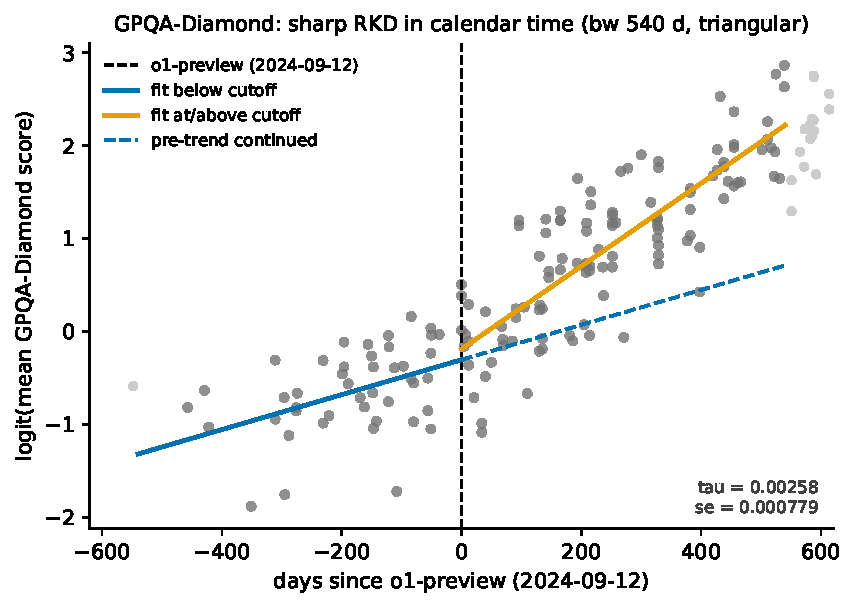
\includegraphics[width=0.82\linewidth]{fig_gpqa}
\caption{GPQA-Diamond, logit(mean score) against days since o1-preview
(2024-09-12). Solid lines: kernel-weighted local-linear fits on each side
(bandwidth 540 days, triangular); dashed: the pre-cutoff trend continued. The
slope roughly $2.4\times$'s at the cutoff, and the placebo grid (empirical size
0/7) localizes the bend to the date.}
\label{fig:gpqa}
\end{figure}

\subsection{METR time horizon: a real bend that cannot be dated}\label{sec:metr}

The $\log_2$ 50\%-time-horizon slope rises from $0.00331$ to $0.00932$ per day at
bandwidth 720 (triangular): a doubling time of $9.9$ months before the cutoff
falling to $3.5$ months after (Figure~\ref{fig:metr}). The headline kink is
$+0.00601$ (se $0.00282$, $t = 2.13$); the full-sample uniform-kernel fit gives
$+0.00491$ (se $0.00095$, $t = 5.17$; doubling time $7.6 \to 3.6$ months). The
estimate is positive in 8/8 bandwidth$\times$donut cells ($0.0044$--$0.0085$), and
the 80\%-horizon variant agrees ($+0.00454$, $t = 4.08$), though with only three
pre-cutoff points it is directional corroboration only.

But the placebo grid smears on the pre side: at bandwidth 720, shifted cutoffs at
$-270$, $-180$, and $-90$ days all reject ($p = 0.030$, $0.014$, $0.004$) with
estimates the size of the headline kink, while post-side shifts are clean nulls
(empirical size 3/6). With 11--12 pre-cutoff models, adjacent placebo windows share
most of their data, and the design cannot distinguish 2024-09-12 from any date
within roughly $\pm 270$ days on the pre side. The honest verdict, quoted from the
analysis of record: \emph{``credible slope change with failed date-localization ---
report as reasoning-era slope doubling, not `o1-preview caused X'.''} This is the
era-bend/event-bend contrast with Section~\ref{sec:gpqa} in a single dataset pair.

\begin{figure}[t]
\centering
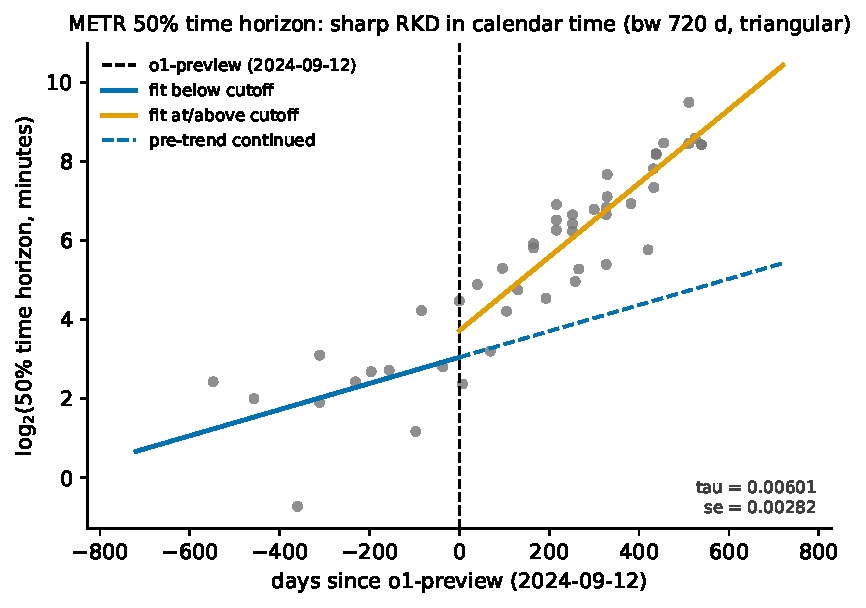
\includegraphics[width=0.82\linewidth]{fig_metr}
\caption{METR 50\% time horizon ($\log_2$ minutes) against days since o1-preview.
The slope nearly triples (doubling time $9.9 \to 3.5$ months at bandwidth 720),
but pre-side placebo cutoffs also reject: an era bend, not a dated event.}
\label{fig:metr}
\end{figure}

\subsection{The Epoch Capabilities Index: a null with power}\label{sec:eci}

If ``everything kinked in 2024'' --- a global measurement or composition shift ---
then per-benchmark kinks would be uninformative. The ECI falsification run was
launched \emph{expecting} a null, and it delivered one: at the o1 date the
all-models kink is null in 8/8 grid cells ($t$ from $-0.60$ to $-1.54$; headline
$-0.00725$ points/day, se $0.00895$), with the index gaining roughly 18 points per
year on both sides of the cutoff (Figure~\ref{fig:eci}). Crucially, the same
series' placebo grid rejects at 4/7 shifted cutoffs --- the test demonstrably has
power in this data, from composition-churn bends elsewhere in the series --- and
still reads zero at 2024-09-12. The instrument works; the dial reads zero. The
per-benchmark bends of Sections \ref{sec:gpqa}--\ref{sec:metr} are therefore not a
global measurement artifact. This is partly by construction (IRT linking smooths
regime shifts) and partly because o1-era gains concentrate in reasoning-heavy
benchmarks.

Two recorded lessons ride along. First, an analyst-script frontier filter ---
\texttt{cummax().diff()} \texttt{.fillna(1) > 0} over a series with 231 NaN
scores --- manufactured 347 false ``frontier records''; the clean frontier has 25 points and
is \emph{not} an estimable design --- four left-cell points, failing donut,
bandwidth-direction, and placebo checks in every direction --- and should never be
quoted. Second, a side finding: the training-compute covariate kink among
ECI-listed models is $-0.00265$ $\log_{10}$ FLOP/day at the o1 date ($p = 0.021$),
corroborating the ``pretraining-compute frontier stalls'' narrative without itself
being a design.

\begin{figure}[t]
\centering
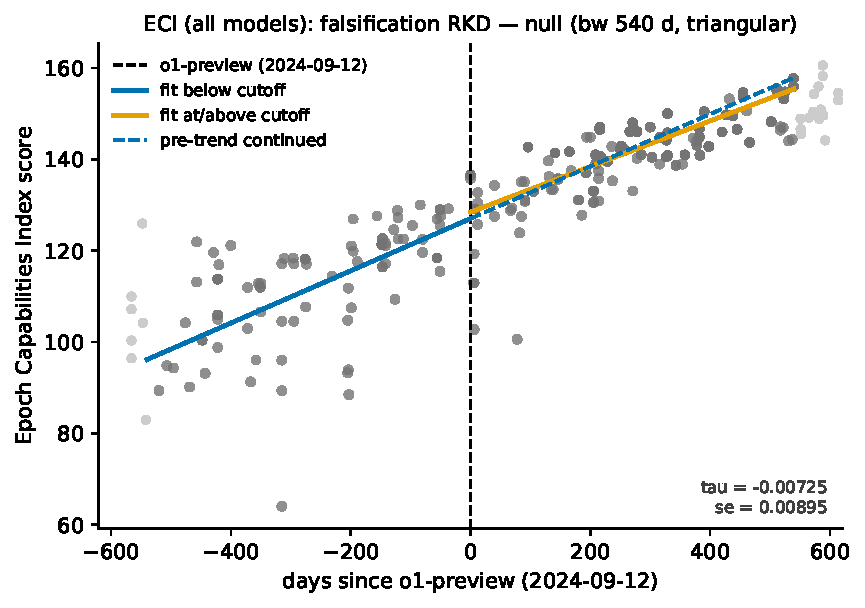
\includegraphics[width=0.82\linewidth]{fig_eci}
\caption{Epoch Capabilities Index (all models) against days since o1-preview. The
two-sided fit and the continued pre-trend nearly coincide: a clean null
($t = -0.81$) in a series where the placebo grid shows the test has power
(4/7 shifted cutoffs reject). The guard the per-benchmark kinks need.}
\label{fig:eci}
\end{figure}

\subsection{China's chip stock at the October 2023 export controls}\label{sec:china}

The only true difference-in-kinks structure in the corpus: the US export-license
schedule bends for China only, at a common dated cutoff (2023-10-17), so treated =
China and control = hyperscalers (Amazon + Microsoft + Google + Meta), and the
controls difference out the global supply bend (their own kink: $-0.00067$/day).
The legal-stock DiK is $-0.00154$ log-units per day (se $0.00047$, $t = -3.30$;
bandwidth 548, triangular), i.e.\ a growth-rate change of roughly
$\mathbf{-0.56}$ \textbf{log-units per year} (Figure~\ref{fig:china}). By-year CR1
clustering keeps significance ($t = -5.15$) with the explicit few-cluster caveat
($G = 4$). The estimate is negative in \textbf{25/25} specifications.

Falsifications behave: the October 2022 first-round placebo --- the round whose
A800/H800 compliance loophole predicts no bite --- is null/positive ($+0.0018$,
$p = 0.15$), and the placebo-treated group (``Other'' vs.\ hyperscalers) is clean
at bandwidths 548--730 while rejecting at 365, so the defensible range is
bandwidth 548--730 with DiK $-0.0009$ to $-0.0015$. The honesty band: the
\emph{total}-stock series including smuggled chips gives a DiK roughly half the
size and fragile ($-0.00076$, $t = -1.54$ at bandwidth 548) --- the smuggled
series, which starts 2024-03-31 and is itself a treatment response, substitutes
for lost legal supply. Serial dependence in a six-points-per-cell cumulative
series makes every $|t|$ optimistic; the sign stability is the real evidence. The
verdict of record: \emph{``the policy bent the legal channel $\approx -0.3$ to
$-0.56$ ln-units/yr; the effect on China's actual compute stock is smaller and
fragile.''}

\begin{figure}[t]
\centering
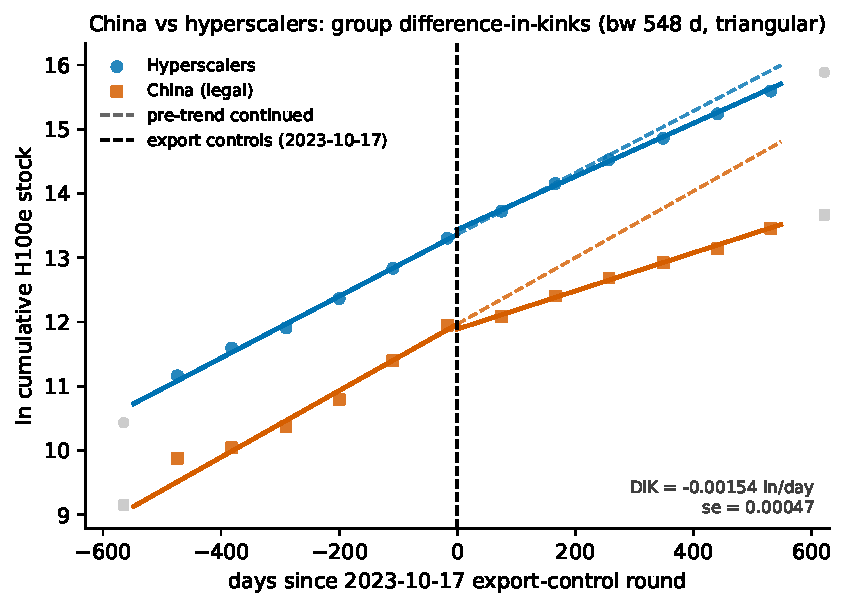
\includegraphics[width=0.82\linewidth]{fig_china}
\caption{Group difference-in-kinks: $\ln$ cumulative H100e stock for China
(legal) and the hyperscaler controls against days since the 2023-10-17
export-control round (bandwidth 548 days, triangular). Both series bend at the
cutoff; the DiK is their difference, $-0.00154$ log-units/day
($\approx -0.56$/yr).}
\label{fig:china}
\end{figure}

\section{The graveyard}\label{sec:graveyard}

Rejections are results. Three claims that look at least as impressive as
Table~\ref{tab:headline} in a scatter plot died in the battery.

\paragraph{Datacenter growth ``kinked at ChatGPT.''}
The GPU-cluster series ($\ln$ cumulative H100e by first-operational date) shows a
nominal kink at ChatGPT's release with $t = 12.9$ --- the largest $t$-statistic of
the entire exercise. Its placebo grid rejects at \textbf{7/7} shifted cutoffs
(empirical size $1.0$): a smoothly super-exponential cumulative series bends
\emph{everywhere}, and HC1 inference on serially dependent cumulative data is
meaningless. The design was discarded; the estimate is descriptive curvature, not
a kink. (The dataset variant named in the original claim, datacenter power
timelines, was infeasible outright: one pre-ChatGPT observation.) This is the
cautionary tale for every ``the curve bent at [event]'' plot drawn on cumulative
infrastructure data.

\paragraph{Chinchilla.}
Tokens-per-parameter among language base models at the Chinchilla paper's release
date (2022-03-29): kink $t = -0.91$, $-0.05$, $+1.48$ at bandwidths 365, 540, 730
--- a sign-unstable null. Even a genuine regime change (prior work shows a two-to-three-month
adoption ramp) does not produce a slope kink dateable to the paper's release.

\paragraph{The EU AI Act threshold is a step with bunching, not a kink.}
The Act's systemic-risk presumption at $10^{25}$ training FLOP imposes a
\emph{level} discontinuity in obligations, not a marginal-rate kink, so RKD/DiK is
the wrong estimand shape. Worse for any kink or RD design at that cutoff, the
running variable sorts: post-Act, the model-density just above the line is
depleted (below/above contingency: Fisher exact $\mathrm{OR} = 0.17$, 95\% CI
$0.05$--$0.62$, $p = 0.0071$; roughly 83\% of the expected above-line mass
missing), which violates any no-sorting requirement. Kink-shaped probes confirm
nulls (e.g.\ an open-weights-share DiK of $-0.93$, se $0.72$). The bunching test
remains the right tool at this threshold --- and the bunching itself, an
avoidance response specific to the statutory line and the post-Act period, is the
substantive finding.

\section{Discussion}\label{sec:discussion}

Four lessons generalize beyond these datasets.

\textbf{Era bends and event bends are different claims.} The METR and GPQA series
tell almost the same visual story --- capability slopes steepen around late 2024
--- yet the placebo grid cleanly separates them: GPQA's bend localizes to the o1
date (size 0/7) while METR's does not (pre-side size 3/6). Public discussion
rarely distinguishes ``the trend changed in this era'' from ``this event changed
the trend''; the shifted-cutoff grid makes the distinction mechanical.

\textbf{Nulls need power certificates.} The ECI falsification is informative
precisely because the same series rejects at 4/7 shifted placebo cutoffs: the
test has power in this data, and still reads zero at the candidate date.
A null from an underpowered test would have guarded nothing.

\textbf{Report honesty bands, not point claims.} The China result is strongest as
a band: legal-channel bend $\approx -0.3$ to $-0.56$ log-units/yr across the
defensible bandwidth range, total-stock effect roughly half and fragile because
smuggling --- itself a response to the policy --- substitutes for legal supply.
Similarly, GPQA's $\tau$ is a release-stream property with composition as the
mechanism, not per-model improvement.

\textbf{The graveyard is the argument.} The most significant statistic of the
exercise ($t = 12.9$) belongs to a design that fails every placebo. Any workflow
that stops at ``the kink is significant'' would have led with it. On the public
record of AI progress, where series are short, serially dependent, and
composition-churned, the falsification battery is not a robustness appendix ---
it is the analysis.

\emph{Limitations.} Calendar-time identification rests on an untestable
no-co-located-event assumption; placebo grids probe but cannot certify it. Several
series are short (6 quarterly points per cell in the DiK; 11--12 pre-cutoff models
for METR), making serial dependence corrections coarse and $|t|$ optimistic.
Epoch's compute figures are partly estimates, and benchmark contamination drifts
over time. All results are properties of the \emph{public record} of AI progress
--- release-stream composition included --- not of any individual system.

\subsection*{Reproducibility}

Estimates were produced with the open-source \natex{} v0.2.0 kink module
\cite{natex} on public Epoch AI data \cite{epochdata}; the per-design analysis
records (inputs, CLI outputs, diagnostics JSON) and the case-study write-up of
record live in the \natex{} repository under
\texttt{docs/case\_studies/} (\texttt{epoch-kinks.md}). The four figures
regenerate deterministically from the public CSVs via the committed script
\texttt{paper/figures/} \texttt{make\_figures.py}, which asserts every headline
number against the case study before drawing.

\begin{thebibliography}{9}

\bibitem{bockerman2025}
B\"ockerman, P., Jysm\"a, S., and Kanninen, O. (2025).
\emph{Difference-in-Kinks Design}.
IZA Discussion Paper No.~18313.
\url{https://docs.iza.org/dp18313.pdf}

\bibitem{herlands2018}
Herlands, W., McFowland~III, E., Wilson, A.~G., and Neill, D.~B. (2018).
Automated local regression discontinuity design discovery.
In \emph{Proceedings of the 24th ACM SIGKDD International Conference on Knowledge
Discovery and Data Mining (KDD~'18)}.

\bibitem{epochdata}
Epoch AI (2026).
Data on AI: AI Benchmarking Hub, Epoch Capabilities Index, and AI chip data.
Published online at \url{https://epoch.ai/data}. Retrieved July 2026. CC-BY 4.0.

\bibitem{natex}
Hillebrandt, H. (2026).
\emph{natex: automated natural-experiment discovery and estimation} (version
0.2.0). Software.
\url{https://github.com/HaukeHillebrandt/natex}

\bibitem{kwa2025}
Kwa, T., West, B., Becker, J., et al. (2025).
Measuring AI ability to complete long tasks.
arXiv:2503.14499.

\bibitem{rein2023}
Rein, D., Hou, B.~L., Stickland, A.~C., et al. (2023).
GPQA: A graduate-level Google-proof Q\&A benchmark.
arXiv:2311.12022.

\end{thebibliography}

\end{document}
